\documentclass[11pt]{beamer}
\usepackage[OT1]{fontenc}
\usepackage[utf8x]{inputenc}
\usepackage[frenchb]{babel}
%\usepackage[dvipsnames]{xcolor}
\usepackage{xcolor}
\usetheme{PickEM}
\title{D\'eveloppement d'un utilitaire de s\'election de particules observ\'ees au microscope \'electronique}
\subtitle{Pick\_EM}
\date{Mai 2012}
\author{\textsc{Faux} - \textsc{Héricé} - \textsc{Paysan-Lafosse} - \textsc{Sansen}}
\institute[Universite Bordeaux 1 \& 2] 
{
 Master 1 Bioinformatique \\ Projet de programmation sous la direction de Jean-Christophe \textsc{Taveau} \\ 
 \begin{figure}[h]
  \begin{center}
  
\includegraphics[width=0.25\columnwidth]{beamer/logounibdx.png}
  \hspace{1cm}
  
\includegraphics[width=0.3\columnwidth]{beamer/banniere_cbmn.png}
  \end{center}
 \end{figure}
}

%\AtBeginSection[]{
%  \begin{frame}{Plan}
%  \small \tableofcontents[currentsection, hideothersubsections]
%  \end{frame} 
%} 
 
\begin{document}

\frame{\titlepage}
\section*{Sommaire}
\begin{frame}
  \tableofcontents
\end{frame}
\section{Introduction}
\begin{frame}
\frametitle{\secname}
\begin{block}{CBMN}
Laboratoire de Chimie et Biologie des Membranes et Nanoobjets 
\end{block}
\begin{block}{ACMPC}
\'Equipe Architectures des Complexes Membranaires et Processus Cellulaires
\end{block}
\end{frame}

\subsection{Contexte}
	\begin{frame}
	\frametitle{\subsecname}
	\begin{itemize}
		\item Micrographies de structures protéiques issues de MET
		\item Utilisation du logiciel ImageJ
		\item Sélection manuelle fastidieuse 
		\begin{itemize}
			\item Chronophage
			\item Accapare un membre de l'équipe
			\item Répétitive
		\end{itemize}
	\end{itemize}
	\begin{figure}
		\includegraphics[scale=0.05]{beamer/base.jpg}
		
		Exemple de micrographie
	\end{figure}
\end{frame}

\subsection{Objectifs}
\begin{frame}
\frametitle{\subsecname}
	\begin{columns}[t]
		
		\begin{column}{4.5cm}
			\begin{block}{Création d'une interface}
				\begin{itemize}
					\item Facile d'utilisation
					\item Claire et succincte
					\item Récupération des paramètres utilisateurs
				\end{itemize}
			\end{block}
		\end{column}
		\begin{column}{6.5cm}
		    \begin{block}{Implémentation d'algorithmes}
				\begin{itemize}
					\item Automatisation du traitement et de la sélection
					\item Récupération des coordonnées
					\item Images individuelles
				\end{itemize}
			\end{block}
		\end{column}
	\end{columns}
\end{frame}

\section{Analyse}
\subsection{Besoins fonctionnels}
\begin{frame}
\frametitle{\subsecname}
	\begin{columns}[t]
		
		\begin{column}{5cm}
			\begin{block}{Interface}
				\begin{itemize}
					\item Choix entre plusieurs algorithmes
					\item Diffère entre chaque algorithme
				\end{itemize}
			\end{block}
		\end{column}
		\begin{column}{5cm}
			\begin{block}{Algorithmes}
				\begin{itemize}
					\item Sélection automatique
					\item Résultats : tableau de coordonnées (x, y, z) et pile d'images individuelles
				\end{itemize}
			\end{block}
		\end{column}
	\end{columns}	
\end{frame}

\subsection{Besoins non fonctionnels}
\begin{frame}
\frametitle{\subsecname}
	\begin{columns}[t]
		\begin{column}{5cm}
			\begin{block}{Interface}
				\begin{itemize}
					\item Implémentation en Java (AWT ou \textbf{Swing})
					\item Modularité
				\end{itemize}
			\end{block}
		\end{column}
		\begin{column}{5cm}
			\begin{block}{Algorithmes}
				\begin{itemize}
					\item Implémentation en Java (tests avec l'outil Macro d'ImageJ)
					\item Traitement rapide (grands jeux de données)
					\item Minimiser les étapes intermédiaires
				\end{itemize}
			\end{block}
		\end{column}
	\end{columns}
\end{frame}

\section{Conception - Réalisation}
\subsection{Interface Graphique (GUI)}
\begin{frame}
\frametitle{\subsecname}
	\begin{columns}
		\begin{column}{6cm}
			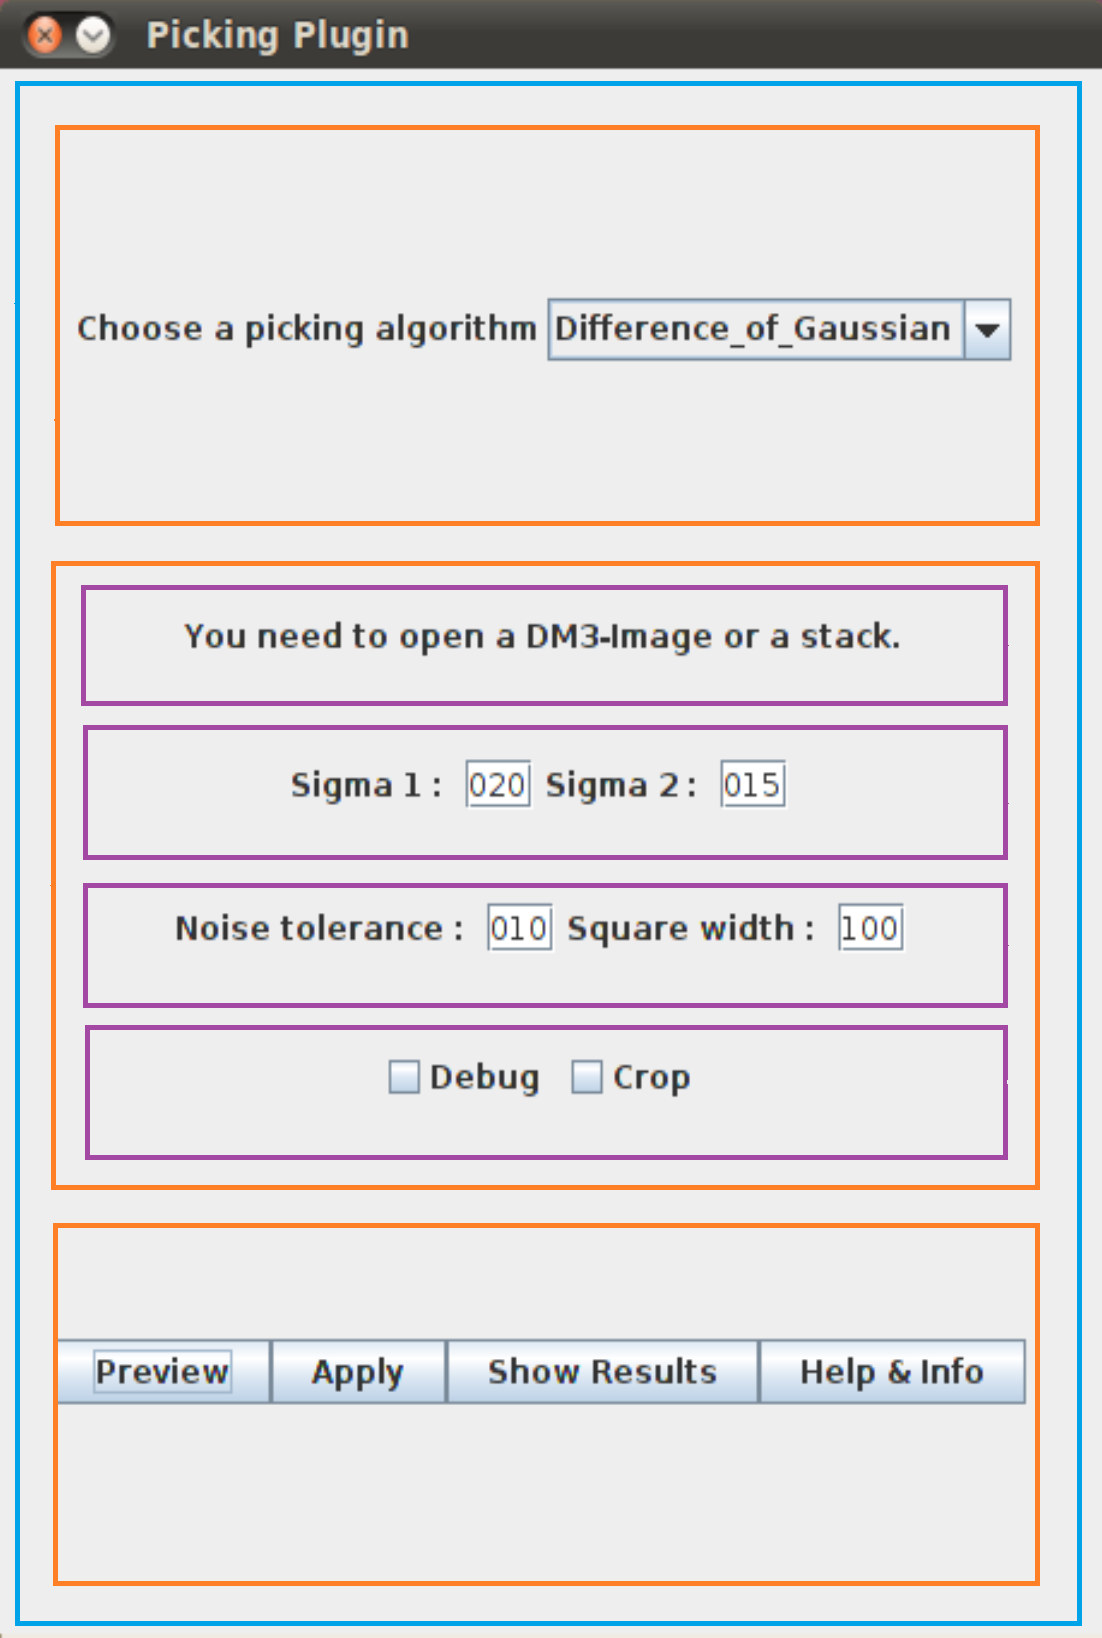
\includegraphics[scale=0.12]{beamer/pluginCadres.png}
		\end{column}
		\begin{column}{4cm}
			Organisation générale de l'interface
		\end{column}
	\end{columns}
\end{frame}
\subsubsection*{Récupération des paramètres utilisateurs}
\begin{frame}
\frametitle{GUI - \subsubsecname}
	%Patrons de Conception : \emph{Factory} et \emph{Singleton}
	\begin{columns}[t]
		\begin{column}{5cm}
			\begin{block}{Choix de l'algorithme}
				\begin{itemize}
					\item JComboBox
				\end{itemize}
			\end{block}
			\vspace*{2cm}
			\includegraphics[scale=0.45]{beamer/combobx.png}
		\end{column}
		\begin{column}{5cm}
			\begin{block}{Paramètres propres aux algorithmes}
				\begin{itemize}
					\item JTextField
					\item JCheckBox
				\end{itemize}
			\end{block}
			\includegraphics[scale=0.15]{beamer/param.png}
		\end{column}
	\end{columns}
\end{frame}
\subsection{Algorithmes}
\subsubsection*{Les agorithmes implémentés}
\begin{frame}
\frametitle{\subsubsecname}
\begin{block}{3 algorithmes implémentés:}
\begin{itemize}
\item Extraction de contours (Différence de dilatation)
\item Corrélation d'images
\item Différence de Gaussiennes 
\end{itemize}
\end{block}
\end{frame}
\begin{frame}
\frametitle{\subsecname ~- Extraction de contours}
\begin{columns}
		\begin{column}{5cm}
			\begin{figure}
				\includegraphics[scale=0.5]{beamer/blobs-1.png}

				Image après dilatation
			\end{figure}
		\end{column}
		\begin{column}{5cm}
		%\begin{figure}
	%	\includegraphics[scale=0.02]{beamer/rond.png}

	%		cercle de comparaison
	%\end{figure}
			\begin{figure}
				\includegraphics[scale=0.5]{beamer/blobDilateDiffResult.png}

				Image résultante
			\end{figure}
		\end{column}
	\end{columns}
\end{frame}
\begin{frame}
\frametitle{\subsecname ~- Corrélation d'images}
	\begin{columns}
		\begin{column}{5cm}
			\begin{figure}
				\includegraphics[scale=0.07]{beamer/exemple.png}

				Image pour la corrélation
			\end{figure}
		\end{column}
		\begin{column}{5cm}
		%\begin{figure}
	%	\includegraphics[scale=0.02]{beamer/rond.png}

	%		cercle de comparaison
	%\end{figure}
			\begin{figure}
				\includegraphics[scale=0.07]{beamer/Result.png}

				Image résultante
			\end{figure}
		\end{column}
	\end{columns}
\end{frame}
\subsubsection*{Démonstration avec la Différence de Gaussiennes}
\begin{frame}
\frametitle{\subsubsecname}%(DoG) Wouf!}
%	\begin{columns}
%		\begin{column}{5cm}
			\begin{figure}
				\includegraphics[scale=0.09]{beamer/base.jpg}
	
				Micrographie de protéines transmembranaires
			\end{figure}
%		\end{column}
%		\begin{column}{5cm}
%			\begin{itemize}
%				\item Application de filtres gaussiens
%				\item Soustraction des images filtrées
%				\item Récupération des maxima
%				\item Extrapolation des points sélectionnés sur l'image de bases
%			\end{itemize}
%		\end{column}
%	\end{columns}
\end{frame}
\begin{frame}
\frametitle{\subsecname ~- Les filtres}
%\begin{center}
Application de filtres gaussiens
%\end{center}
	\begin{columns}
		\begin{column}{5cm}
			\begin{figure}
				\includegraphics[scale=0.07]{beamer/filtreGaussien15.jpg}
				
				Filtre Gaussien (Radius 15)
			\end{figure}			
		\end{column}
		\begin{column}{5cm}
			\begin{figure}
				\includegraphics[scale=0.07]{beamer/filtreGaussien20.jpg}
				
				Filtre Gaussien (Radius 20)
			\end{figure}
		\end{column}
	\end{columns}
\end{frame}
\begin{frame}
\frametitle{\subsecname ~- Résultats intermédiaires}
%\begin{center}
Soustraction des images filtrées et Récupération des maxima
%\end{center}
\begin{columns}
\begin{column}{5cm}
			\begin{figure}
				\includegraphics[scale=0.07]{beamer/resultsubstractgaussian.jpg}
				
				Résultat de la soustraction
			\end{figure}
\end{column}
\begin{column}{5cm}
			\begin{figure}
				\includegraphics[scale=0.14]{beamer/gaussianmaxima.jpg}
				
				Résultat du maxima
			\end{figure}
\end{column}
\end{columns}
\end{frame}
\begin{frame}
\frametitle{\subsecname ~- Résultats}
Application des points d'intérêt sélectionnés sur l'image de bases
	\begin{columns}
		\begin{column}{5cm}
			\begin{figure}
				\includegraphics[scale=0.13]{beamer/imgCrop.png}
				
				Résultat du piquage
			\end{figure}
		\end{column}
		\begin{column}{5cm}
			\begin{figure}
				\includegraphics[scale=0.12]{beamer/cropall.png}
				
				Images individuelles et tableau de coordonnées
			\end{figure}
		\end{column}
	\end{columns}
\end{frame}
\subsection{Modularité}
\subsubsection*{Diagramme de classes}
\begin{frame}
\frametitle{\subsecname ~- \subsubsecname}
	\begin{figure}
		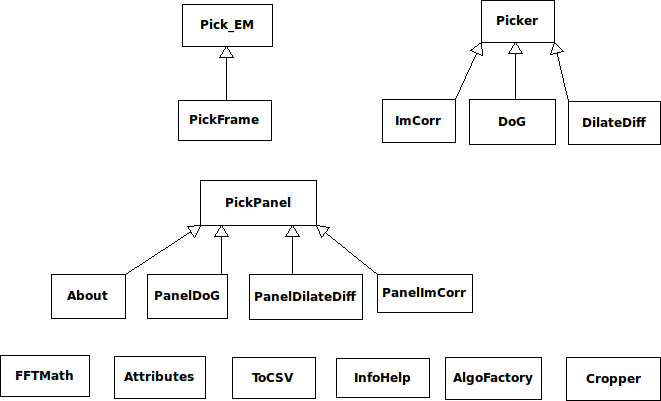
\includegraphics[scale=0.4]{beamer/class_diagram.png}
				
		Diagramme des classes
	\end{figure}
\end{frame}
\subsubsection*{Patrons de conception}
\begin{frame}
\frametitle{\subsecname ~- \subsubsecname}
	\begin{block}{Singleton}
		\begin{itemize}
			\item Sert à contrôler le nombre d'instances d'une classe présent à un moment donné
			\item Restreint l'instanciation d'une classe à un seul objet
		\end{itemize}
	\end{block}
	\begin{block}{Factory}
		\begin{itemize}
			\item Classe qui n'a pour rôle que de construire des objets
			\item Seule responsable de la création $/$ distribution de l’objet
		\end{itemize}
	\end{block}
\end{frame}
\begin{frame}
\frametitle{Difficultés rencontrées}
	\begin{block}{API ImageJ}
	Distinction :
		\begin{itemize}
			\item ImagePlus
			\item ImageProcessor
			\item ImageStack
		\end{itemize}
	\end{block}
	\begin{block}{GUI}
		\begin{itemize}
			\item Gestion des panneaux
			\item Organisation et tailles des fenêtres
		\end{itemize}
	\end{block}
\end{frame}
\begin{frame}
\frametitle{Améliorations}
	\begin{block}{Améliorer:}
		\begin{itemize}
			\item Améliorer le mode Debug
			\item Continuer le travail pour l'utilisation en Macro
		\end{itemize}
	\end{block}
	\begin{block}{Ajouter :}
		\begin{itemize}
			\item Ajouter automatiquement un algorithme
			\item Afficher les sélections pour chaque image d'une pile
		\end{itemize}
	\end{block}
\end{frame}
\section{Conclusion}
\begin{frame}
\frametitle{\secname}
%Travail sympa, équipe cool, collègue parfois relou Taveau change tout le temps d'idée
	\begin{block}{Le projet}
		\begin{itemize}
			\item Interface facile d'utilisation
			\item Sélection efficace
			\item Récupération fonctionnelle des images individuelles et des coordonnées 
		\end{itemize}
	\end{block}
	\begin{block}{L'équipe}
		\begin{itemize}
			\item Première expérience de travail en équipe sur un gros projet concluante
			\item Aperçu de notre futur métier
		\end{itemize}
	\end{block}
\end{frame}
\begin{frame}
	\frametitle{}
	\begin{block}{}
		\begin{center}
			Merci beaucoup pour votre attention ! %votez jean bon!
		\end{center}
	\end{block}
\end{frame}

\end{document}